\documentclass[3p,times]{elsarticle}
\usepackage{amsmath}
\usepackage{amsfonts} %potrzebne do \mathbb{S}
\usepackage{here}
\usepackage{caption}
\usepackage{subcaption}
\usepackage{color}
\def\spe{\mathbf{Spec}}
\usepackage{graphicx}
\usepackage{soul}   %package for highlight
\newcommand{\noop}[1]{}
\newtheorem{problem}{Problem}
\usepackage{lineno,hyperref} 
\modulolinenumbers[5]
\journal{Measurement}
\usepackage{multirow}
\usepackage{blindtext}
\usepackage{pict2e}
\newenvironment{thisnote}{\par\color{blue}}{\par}
\newenvironment{rednote}{\par\color{red}}{\par}
%% `Elsevier LaTeX' style
%\bibliographystyle{abbrvnat}%\biboptions{sort&compress}
\bibliographystyle{elsarticle-num}\biboptions{sort&compress}
%%%%%%%%%%%%%%%%%%%%%%%

\begin{document}

\begin{frontmatter}

\title{Local damage detection based on vibration data analysis in the presence of Gaussian and heavy-tailed impulsive noise}


%% Group authors per affiliation:
\author[label1]{Jacek Wodecki}
\author[label1]{Anna Michalak \corref{cor1}}
\cortext[cor1]{Corresponding author, anna.michalak@pwr.edu.pl}
\author[label1]{Rados{\l}aw Zimroz}
% \author[label2]{Agnieszka Wy{\l}oma{\'n}ska}

\address[label1]{Faculty of Geoengineering, Mining and Geology, Wroclaw University of Science and Technology, Na Grobli 15, 50-421 Wroclaw, Poland
\\\{jacek.wodecki, anna.michalak radoslaw.zimroz\}@pwr.edu.pl\\}
% \address[label2]{Faculty of Pure and Applied Mathematics, Hugo Steinhaus Center, Wroclaw University of Science and Technology,Wybrze{\.z}e Wyspia{\'n}skiego 27, 50-370 Wroclaw, Poland
% \\ agnieszka.wylomanska@pwr.edu.pl\\}

\begin{abstract}

Local damage detection in bearings focuses on the identification of periodically impulsive components. Popular methods assume presence of either non-Gaussian noise or different frequency band for informative and non-informative impulses, and use statistics to select appropriate band. Here two impulsive sources occupy the same frequency range: a fault-related signal of interest, and non-cyclic noise describing random events during particular technological process (crushing, sieving etc.). The task is formulated as damage detection in presence of non-Gaussian impulsive noise. We propose to use Nonnegative Matrix Factorization of spectrogram for separation of cyclic and non-cyclic impulsive components. Partial information is fused into a single data set for each component. Finally, post-processing is implemented to allow to recover the time series of each component. New method allows to detect and extract impulsive signal (damage in bearing) in presence high amplitude non-cyclic impulsive signal. Moreover, the algorithm allows to properly indicate lack of any damage.

\end{abstract}




\begin{keyword}
Nonnegative Matrix Factorization, beta-divergence, local damage detection, time-frequency representation, phase reconstruction, vibration, ore crusher
\end{keyword}

\end{frontmatter}

\linenumbers

\section{Introduction}

Real-life vibration signals are typically nonstationary, noisy and contain weak damage related signature \cite{maheswari2017trends}. As a first step, the informative frequency band selection (IFB) is a common way to pre-filter raw data and then detect the damage in such scenario \cite{li2016fuzzy,jin2018informative}. IFB refers to the frequency band which is occupied by the information about damage which is relatively easy to identify (Signal to Noise Ratio is high enough to detect damage). One of the most popular method in this direction is filtration with spectral kurtosis \cite{antoni2006spectral,combet2009optimal} or other selectors such as conditional variance selector \cite{HebdaSobkowicz2020b}, optimal filters \cite{wodecki2018optimal}, or selectors based on other statistics \cite{obuchowski2014selection,zak2015application}. Another way of investigating IFB is the approach of kurtogram \cite{antoni2007fast} and other similarly derived representations based on discrete division of frequency spectrum \cite{HebdaSobkowicz2020b,wang2018some} such as spectral Gini index \cite{miao2017improvement_GINI}, IFBI$\alpha$-gram \cite{schmidt2020methodology}, infogram \cite{antoni2016info}, spectral smoothness index \cite{bozchalooi2007smoothness} or harsogram \cite{zhao2016detection}. Besides already mentioned methods, there exist other approaches based on frequency-domain analysis \cite{dybala2018diagnosing,obuchowski2016blind,zhang2015novel}.


Unfortunately the case becomes much more complicated when additional highly energetic impulsive components not related to damage are present in the signal. In this case most of the methods fail, because they focus on this random component and not on the cyclic fault signature that is typically weak in energy. There are however several methods for IFB detection, or in general selector construction, that can handle such situations, however in cases presented therein the frequency bands of fault component and artifact component do not overlap in the most part \cite{HebdaSobkowicz2020b,zak2015application,miao2017improvement_GINI,antoni2016info,Borghesani2017}. 
All of those techniques have some advantages and limitations. On the other hand, it is much more difficult when the frequency band of the both components overlap completely, or even the band of random component is the wider one. In such case it is impossible to separate those components based on the frequency-domain analysis.
 
Furthermore researchers try to take advantage of the periodic aspect of the signal components in interesting ways. For example, a periodically varying filter is used for fault indication \cite{kruczek2017cyclic}. Periodicity is one of the reasons that the popular approach is to use multidimensional data representations, specifically time-frequency domains or bi-frequency representations, i.e. spectral coherence \cite{randall2011rolling}. One of the interesting approaches for time-frequency analysis of rotating machinery is described \cite{feng2013recent}. There are also numerous papers published on the topic of cyclostationary analysis of vibration signals in the diagnostics of machines operating in a cyclic way \cite{Borghesani2017,antoni2009cyclostationarity,wodecki2019impulsive,biedka1996robust,zhao2019rolling}. 


Another approach has been presented to deal with such situation, and it is based on the fractional moments analysis \cite{zak2017alpha}. Fractional lower-order covariance map (FLOC) has been used to observe the periodicity of the fault-related component. Similar approach applying dependency measures to time-frequency representation has been proposed \cite{kruczek2020detect}. Another use of fractional lower order statistics has been also proposed \cite{ma1996joint}.

Unfortunately, those methods focus only on the fact of periodicity and cannot return the time series of a component as a result, so neither the fault component can be extracted and observed, nor the random impulsive component can be further studied. On the other hand, IFB-oriented methods, or generally speaking frequency-domain analysis will not be able to properly process more difficult data, such as the one presented in this paper, because if frequency bands of components overlap, they will not be separable via spectrum selection.


The approach presented in this paper is a next step of the work on utilizing the idea of Nonnegative Matrix Factorization (NMF) as a tool for damage detection based on vibration data analysis \cite{mehmood2013kernel,liang2019sparse,liang2020impulse,gu2020multi}. Several papers have been already published by the authors in this area \cite{wodecki2017local,wodecki2019novel,wodecki2019impulsive}. The novelty of approach presented in this article is the ability to deal with data that is especially difficult to analyze, namely containing non-cyclic impulsive components where the impulses occur randomly in time and energy, with the frequency spectrum overlapping the informative frequency band that contains the fault-related component. The perfect example of such data is a vibration signal recorded on the hammer ore crusher that operates in the mining industry, which is the signal presented in this paper as test data.

As a result, this method presents several benefits. Using Generalized Hierarchical Alternating Least Squares Nonnegative Matrix Factorization with Beta-Divergence (further referred to as $\beta$-HALS NMF) algorithm allows to construct selective feature set even in the scenario of overlapping frequency bands of the individual signal components. Method is also able to deal with unknown amount of the components hidden in the signal because of using Density-based spatial clustering of applications with noise (DBSCAN) - a robust clustering method that does not require to specify the number of classes. Furthermore the presented approach can automatically associate and label features to allow to reconstruct the individual signal components. As a consequence, in the output it is known what types of components have been discovered in the data, and most importantly, whether the signal contains the fault-related component or not, which is a true-false type of information if the machine is healthy or damaged. Finally, the algorithm reconstructs all components in the from of time series, which enables further investigation. All of the aspects mentioned above can be considered beneficial when using the presented method, since many methods do not exhibit those features.



\section{Methodology}\label{meth} 
\begin{figure}[ht!]
\centering
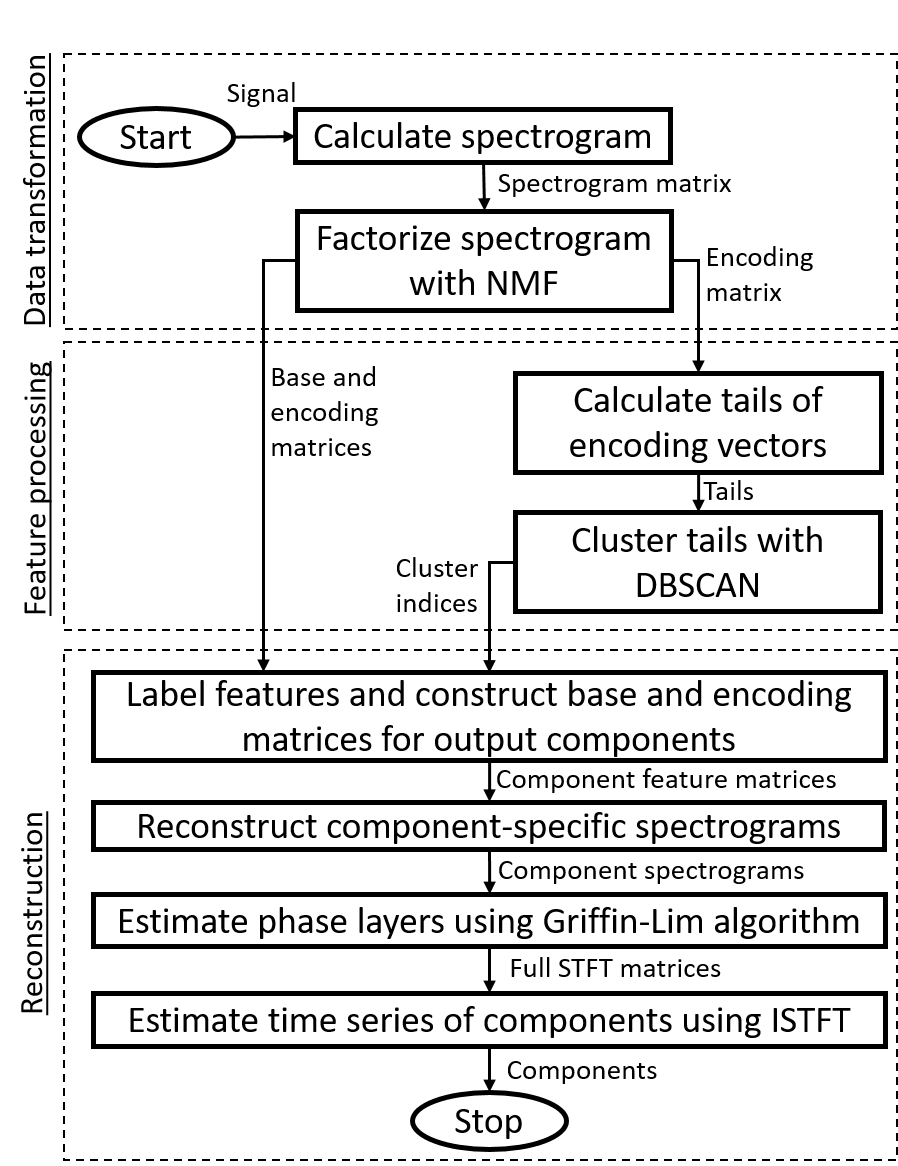
\includegraphics[width=0.65\textwidth]{figs/block.png}
\caption{Flowchart of the presented algorithm.}
\label{fig:block}
\end{figure}
The procedure consists of three main stages: 

\begin{itemize}
 \item \textbf{Data transformation -} this is a preprocessing stage when the algorithm is preparing the required data structures for the actual structural
 analysis. First, for the raw vibration time series from the hammer crusher, a spectrogram is calculated (section \ref{s:sec_spec}). Next, it is factorized using $\beta$-HALS NMF algorithm (section \ref{s:nmf}), which produces two feature matrices (called \emph{base} and \emph{encoding} matrices).
 
 \item \textbf{Feature processing -} in this stage the automatically classification of the features (vector pairs from base and encoding matrices) are presented. Those pairs are grouped based on the analysis of distribution tails of the encoding features using DBSCAN clustering algorithm (section \ref{s:dbscan}). After the indexing of the features, they are taken from the original feature matrices and assembled into new ones for each class (section \ref{s:rec}).

 \item \textbf{Reconstruction -} at this stage, each of the components are identified and reconstructed. Based on the identification procedure the appropriate labels are assigned. For each class, according to the NMF model (eq. (\ref{eq:NMF})), its specific spectrogram is estimated. Then, the Griffin-Lin algorithm is used for the complex phase estimation and allows to transform the spectrograms back to the time series and produces the reconstructed signal components.
\end{itemize}

More detailed description of the algorithm flow is presented on the block diagram (see Fig. \ref{fig:block}).



\subsection{Stage 1: Data transformation}

\subsubsection{Spectrogram}\label{s:sec_spec}

Short-time Fourier transform (STFT) for one-dimensional discrete data $\mathbf{s}$, is defined as \cite{allen1977short}:

\begin{equation}
 \textrm{STFT}(i,k)=\sum_{f=0}^{L-1}s[k+f]w[f]e^{-j2\pi if/I},
\end{equation}
where $f$ is the iterator over the samples within a window, $j$ is the imaginary operator, $0\leq i \leq I-1$ is frequency bin, $k=0,\dots,K-1$ is time point, and $w[.]$ is the window of length $L$. The spectrogram is an absolute value of the STFT:

\begin{equation}
\label{eq:spec_Y}
Y(i,k)=\textrm{Spec}(i,k)=|\textrm{STFT}(i,k)|.
\end{equation}



\subsubsection{Generalized Hierarchical Alternating Least Squares Nonnegative Matrix Factorization with Beta-Divergence}\label{s:nmf}

 
In the wide variety of matrix factorization techniques there exists a group of Nonnegative Matrix Factorization methods. Their most important common feature is that both input matrix and output matrices cannot have negative entries. This particular feature makes those algorithms appropriate for the analysis of data structures that describe energy in some way, since the energy values are always nonnegative. Particular NMF procedure used in this paper is used for the factorization of a magnitude spectrogram.

The NMF model considered in this paper, can be described by the following equation \cite{cichocki2009nonnegative}:

\begin{equation}
  \label{eq:NMF} 
  \mathbf{Y}=\mathbf{AX}+\mathbf{E} = \mathbf{AB}^\textrm{T} +\mathbf{E},
\end{equation}
where $\mathbf{Y}=[y_{ik}] \in \mathbb{R}^{I\times K}$ is the non-negative input spectrogram matrix, defined in (\ref{eq:spec_Y}) $\mathbf{A} = [\mathbf{a}_1, \dots, \mathbf{a}_J] \in \mathbb{R}_+^{I\times J}$ is the unknown base matrix with non-negative vectors $\mathbf{a}_j$, $\mathbf{X}=\mathbf{B}^\textrm{T} = [\mathbf{b}_1,\dots, \mathbf{b}_J]^\textrm{T} \in \mathbb{R}_{+}^{K\times J}$ is the unknown encoding matrix with non-negative components $\mathbf{b}_j^\textrm{T}$, $j=1,\dots,J$ where $J$ is the NMF rank, and $\mathbf{E}=[e_{ik}] \in \mathbb{R}^{I \times K}$ is the matrix corresponds to the estimation errors or noise.

The hierarchical aspect of the algorithm, is that it uses a set of local cost functions and minimizes them sequentially (one-by-one). The fast processing speed and local nature of the learning rules make these algorithms appropriate to the large scale datasets \cite{cichocki2008flexible,cichocki2009fast}. The local cost function based on the $\beta$-divergence ($D_\beta(\cdot||\cdot)$) between two nonnegative sequences can be defined as:

\begin{equation} 
\label{eq:beta_equations}
  D_\beta^{(j)}([\mathbf{Y}^{(j)}]_{+} ||\mathbf{a}_j\mathbf{b}_j^\textrm{T})=
\begin{cases}
\sum_{ik} \left(y_{ik}^{(j)} \frac{\left[y_{ik}^{(j)}\right]^\beta - \left[q_{ik}^{(j)}\right]^{\beta}}{\beta} - \frac{\left[y_{ik}^{(j)}\right]^{\beta+1} - \left[q_{ik}^{(j)}\right]^{\beta + 1}}{\beta+1}  \right), \quad \beta>0,\\
\sum_{ik} \left(y_{ik}^{(j)} \ln \left( \frac{y_{ik}^{(j)}}{q_{ik}^{(j)}} \right) -y_{ik}^{(j)}+q_{ik}^{(j)}  \right), \quad \beta=0,\\
\sum_{ik} \left( \ln \left( \frac{q_{ik}^{(j)}}{y_{ik}^{(j)}} \right)  + \frac{y_{ik}^{(j)}}{q_{ik}^{(j)}} -1 \right),  \quad \beta=-1,
\end{cases}
\end{equation}
where $y_{ik}^{(j)} = \left[ y_{ik} - \sum_{p\neq j} a_{ip}b_{kp} \right]_{+}$ and $q_{ik}^{(j)} = \hat{y}_{ik}^{(j)} = a_{ij}b_{kj}$ for $j=1,\dots,J$.

The multiplicative learning algorithm is obtained by calculation the gradient (\ref{eq:beta_equations}) with respect to the elements $a_{ij}$ and $b_{kj}$.
Then, the gradient components are equalized to zero and the simple Hierarchical Alternating Least Squares (HALS) update rules \cite{cichocki2009nonnegative} are obtained. In this way we get the algorithm named HALS with $\beta$-divergence.
These update rules in the generalized vector form can be described as:

\begin{equation}
  \label{eq:beta_up_rules} 
  \mathbf{b}_j \leftarrow \frac{\left( \left[\mathbf{Y}^{(j)\textrm{T}} \right]_{+}\right)\Psi (\mathbf{a}_j) }{\Psi (\mathbf{a}_j^\textrm{T})\mathbf{a}_j}, \quad \quad a_j \leftarrow \frac{\left( \left[\mathbf{Y}^{(j)} \right]_{+}\right)\Psi (\mathbf{b}_j) }{\Psi (\mathbf{b}_j^\textrm{T})\mathbf{b}_j}, \quad (j=1,\dots,J),
\end{equation}
where $\Psi(\mathbf{b})$ is a suitably chosen convex function, and all nonlinear operation are performed element-wise.

 The optimal $\beta$ parameter is 2 (based on the experimental results) and the convex function is $\Psi(\mathbf{b})=\mathbf{b}^{.\beta}$, where rise to the power $\beta$ is the element-wise operation. 

\subsection{Stage 2: Feature processing}

One of the most important aspects of the entire procedure is the way that features produced by the NMF are analyzed and grouped together, which enables forming data structures that can be later used to reconstruct each signal component. This step needs to take into account both separability of features that do not describe the same component, as well as the similarity of the features that do. This is why in this version of the algorithm the clustering procedure is used. However, it is not known how many individual components there are in the signal, so it is crucial to use the algorithm that does not require to specify the number of clusters on the input. This is why the DBSCAN algorithm is used. It analyzes the local densities in the feature space rather than trying to forcefully produce the number of clusters that the user specified. 

\subsubsection{Feature processing for classification}\label{s:ogony}

Features are clustered based on the encoding vectors. However, the vectors cannot be used directly as data samples. It comes from the fact that they represent feature occurrence in time domain. If two features are to be grouped together and they describe different behaviors in the signal (i.e. different artifacts), their encoding vectors will be different from each other, and since timestamps act as dimensions for clustering, those two features will not be grouped together. 

This is why authors decide to use the distribution tails of the normalized encoding vectors and not the vectors themselves. Tails are distribution-related features, so they describe the process but without considering the time aspect. 

A tail is defined as: 

\begin{equation}
  \label{eq:tails} 
  Tail=1-\hat{F}(\textbf{x}_j), \quad j=1,\dots,J
\end{equation}

where $\hat{F}(\cdot)$ is empirical cumulative distribution function, $J$ is the number of NMF classes, and by $\textbf{x}_j$ we understand the j$^{th}$ vector of encoding vectors. In further analysis the logarithm of the right tail is used.


\subsubsection{DBSCAN}\label{s:dbscan}

Density-based spatial clustering of applications with noise (DBSCAN) is a data clustering algorithm proposed in 1996 \cite{ester1996density}. Given a set of points it assigns together points that are placed close to each other, defining cluster as a high-density region in the feature space. It is still one of the most common and most cited clustering algorithms in the scientific literature.


DBSCAN has two input parameters: $\varepsilon$ which is a radius of neighborhood, and \emph{minPts} -- minimal amount of neighboring points to define a core point. As one can see, there is no input parameter specifying the amount of clusters. This is because the operation of the algorithm is fully data-driven and the dense regions are being discovered in the process, so their number cannot be assumed.
The principle of operation of DBSCAN is very simple: 

\begin{itemize}
  \item If within the radius $\varepsilon$ from a given point it is possible to find at least \emph{minPts} points (counted together with the point itself), then this point is considered to be a core point and is a part of the cluster. 
  \item If the point is not a core point, but lies within the radius $\varepsilon$ from a core point, it is said to be directly reachable from core points. It is considered to be an border point and is still a part of the cluster.
  \item Points that do not have any core points as neighbors within the radius $\varepsilon$ are not part of any cluster and are considered to be outliers.
\end{itemize}

Functioning of described rules is visualized in the Fig. \ref{fig:db}.

\begin{figure}[ht!]
\centering
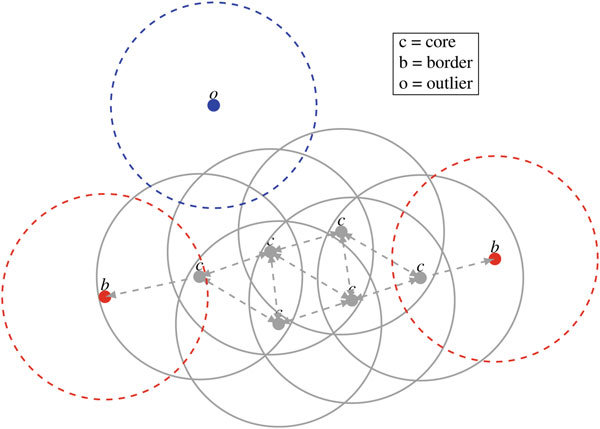
\includegraphics[width=0.7\textwidth]{figs/db1.jpg}
\caption{Visual explanation of DBSCAN. In this diagram, $minPts = 4$. Gray points are core points, because the area surrounding these points in an $\varepsilon$ radius contain at least 4 points in total. Red are not core points, but are reachable from core points and thus belong to the cluster as well. Blue point is a noise point that is neither a core point nor directly-reachable \cite{izzo2016designing}.}
\label{fig:db}
\end{figure}

It is important that a cluster is defined by the presence of core points. For example, if there are two points placed within the radius $\varepsilon$ from each other, but $minPts>2$ and they have no more $\varepsilon$-neighbors, they are both outliers.


\subsubsection{Estimation of the radius $\varepsilon$ for DBSCAN}

The value of the radius $\varepsilon$ is calculated based on the k-nearest neighbor search approach \cite{rahmah2016determination,elbatta2012improvement}. For each point in the dataset, the distance to the $k^{th}$ nearest point is calculated, and the sorted results are plotted. Since datasets considered in this paper are not very numerous, the value $k=3$ is used. Generally, the graph contains a knee. The distance that corresponds to the knee is typically a good choice for $\varepsilon$, because above this value distance between the points exceeds the distances within clusters.

\subsection{Stage 3: Reconstruction}

\subsubsection{Construction of base and encoding matrices}\label{s:rec}

The construction of base and encoding matrices for individual component reconstruction is very simple, because DBSCAN as a clustering algorithm outputs the cluster assignment vector of indices. This vector after reshaping in accordance to the dimensions of input data structure (especially NMF rank) becomes the assignment matrix. At this point base and encoding features belonging to the particular cluster are selected and assembled together to form new base and encoding matrices for each output component. 



\subsubsection{Component labeling}

When data structures for all of the components (noise, damage and artifacts) are assembled, they are labeled. Each of the labels is characterized by the decision rule designed for this component specifically, because different components can be characterized by different behaviors. The analysis is performed on the encoding features of the resulting component obtained by summation of the encoding vectors describing this component. Because of the way that NMF constructs encoding features, there are always small values between the meaningful ones, i.e. there are small non-zero values between impulses in the fault component. In other words, we think about encoding features as binary-style indicators, but in practice they do not contain zeros in places that "do not indicate", but there are always some residue present. To avoid the influence of this effect, especially in the artifact and fault component, the values below $20\%$ of the maximum value of each component are set to 0. The value of $20\%$ has been established based on the distribution analysis of the encoding features. For each component the noise mode tends to separate from the informational part of the distribution around this $20\%$ threshold, so the results have been averaged out to $20\%$. The analysis is based on investigating the behavior of waiting times between the peaks in the signal. This approach is expected to focus on large impulses in the artifact components, cyclic impulses in fault component, and randomly distributed values in the noise component.


\begin{itemize}
  \item \textbf{Artifacts:} Impulses generated by the ore pieces falling into the machine are randomly distributed in time, so this rule operates under two assumptions: 
  \begin{itemize}
    \item There will not be that many high-energy impulses in the 10-second signal;
    \item There will not be a lot of repeating values of waiting times between the high-energy impulses, if any.
  \end{itemize}
  Hence, the rule for detecting artifact component is that there are not more than five repeating values of waiting times between impulses. 
  
  
  % It excludes the fault component in a obvious way, because cyclic component will produce constant values of waiting times (or almost constant, because not every impulse will be sample-accurate in time). Similar case happens with noise component, where detected peaks will be just ordinary local maxima within the noise itself, so there will be a lot of them and a lot will repeat.
  \item \textbf{Noise:} In the noise component the non-zero values are much more numerous and happen rather quickly one after another, so their waiting times distribution
  forms more of a cohesive shape. Since waiting times can take only positive values and for noise a lot of them will be close to zero and not many will be significantly longer, the distribution is expected to be positively skewed. Testing shows that histograms of waiting times for noise fit gamma distribution quite well. The gamma distribution is used to modelling waiting times \cite{guo2011modelling}. Hence, the rule for identifying the noise class is to fit gamma distribution to the waiting times and if the $R^2$ value for the fit quality is larger then 0.9, then the component is labeled as noise.


  \item \textbf{Damage:} Waiting times of peaks in the fault component will focus very tightly around a single value, hence the component is expected to be cyclic. Of course, in practice there will be small deviation of waiting times, because the localization of each impulse in time will not be perfect with zero-sample accuracy. To formalize the presented description the rule is defined that over $60\%$ of waiting times has to take the same value. The value of $60\%$ has been established experimentally based on authors' experience in analyzing various types of diagnostic data originating from the mining industry. In case that period is more irregular (histogram widens even more), histogram of waiting times for the damage component will not fulfill neither of previous rules, which itself acts as a backup rule. An example of such behavior can be observed when diagnosing bearing from the belt conveyor pulley, which is prone to rotation speed deviations \cite{wodecki2018optimal}.

\end{itemize}

\subsubsection{Component reconstruction}

When base and encoding matrices are constructed for each output component, they are multiplied according to the NMF model to obtain the magnitude spectrograms. After that the Griffin-Lim algorithm is applied to estimate the phase layer (imaginary layer) of the complex form of Short-Time Fourier Transform \cite{griffin1984signal}. Finally Inverse Short-Time Fourier Transform (ISTFT) algorithm is used to recover time series of the separated components.

\section{Application to industrial data}

Vibration signal analyzed in this paper is measured on ore crusher operating in the mining industry (see Fig.~\ref{fig:obj_crush}). The signal has been measured on the casing of the rolling-element bearing that holds the main shaft of the machine. It has been acquired with sampling frequency set to 25 kHz using Endevco accelerometers, a data acquisition system was based on NI DAQ interface and Labview Signal Express software. The analyzed vibration signal is 10 s part of the whole measurements. Rotational speed during these parts of the signals might be assumed as approximately constant. Characteristic frequencies of the bearing are presented in Table \ref{tab:freqs}. The considered bearings are 23264 SKF. Due to the analysis presented in Section \ref{case1} the inner race of one bearing reveals a local damage. 

\begin{figure}[ht!]
\centering
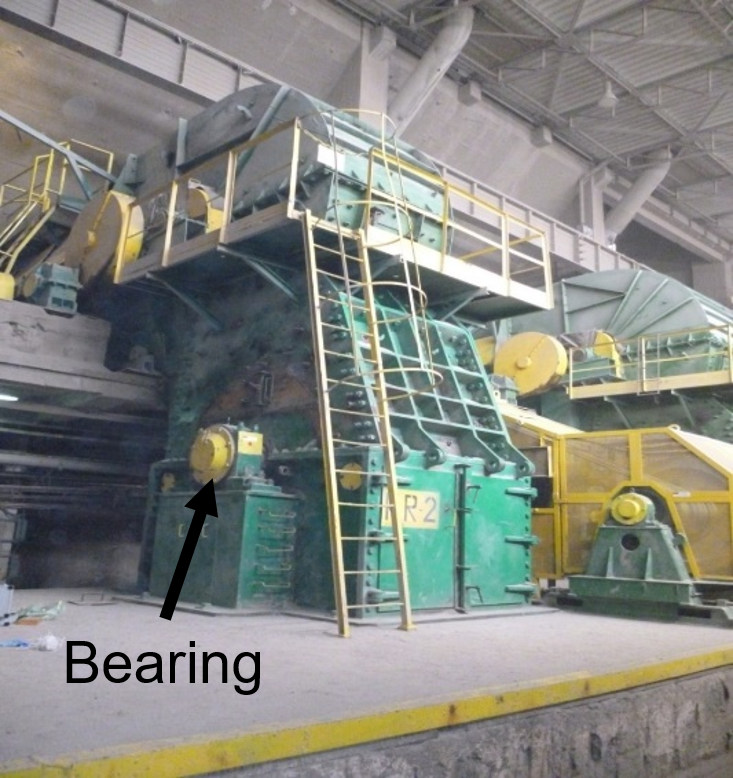
\includegraphics[width=0.5\textwidth]{figs/obj_crush.png}
\caption{Copper ore crusher}
\label{fig:obj_crush}
\end{figure}


\begin{table}[ht!]
  \centering
  \caption{Characteristic frequencies of 23264 CCK/W33 bearing}
  	\resizebox{0.8\textwidth}{!}{
  \begin{tabular}{|l|l|}
  \hline
     \textbf{Description} & \textbf{Value} \\ \hline
     Rotational frequency of the inner ring & 3 Hz\\ \hline
     Rotational freq. of the rolling element and cage assembly & 1.3 Hz\\ \hline
     Rotational freq. of a rolling element about its own axis & 10.6 Hz\\ \hline
     \textbf{Over-rolling frequency of one point on the inner ring} & \textbf{30.7 Hz}\\ \hline
     Over-rolling frequency of one point on the outer ring & 23.3 Hz\\ \hline
     Over-rolling frequency of one point on a rolling element & 21.1 Hz\\ \hline
  \end{tabular}
  }
  \label{tab:freqs}
\end{table}

To test the presented approach two single-channel datasets have been used. The first one contains the signal with artificially introduced fault component modeled after the real faults known from those types of machines, in this case the local damage of the inner race of the bearing, which manifests itself with the characteristic frequency marked in bold in the Table \ref{tab:freqs} \cite{obuchowski2015identification}. In the second dataset the signal from is used directly to test the operation of the algorithm on the data not containing any fault components. Such approach is often used to monitor whether machine is still in good condition.

Another aspect that needs to be tested is the proper operation of the method when there are other components in the signal, such as artifacts or other components that are not similar to the noise and have to be classified separately. Due to the fact that ore falls to the crusher from the top, the impacts of ore pieces generate highly energetic impulses which are random in time and energy, and their spectral structure is different than the one of the noise component. Unfortunately here lies the main difficulty in analyzing such signals: the common frequency band.

Although DBSCAN algorithm used for feature processing works automatically with respect to establishing the number of clusters, as it can be seen based on its description (see section \ref{s:dbscan}), the values of its both parameters are crucial for obtaining proper result of clustering. In this application the value of \emph{minPts} is set to 1. This setting has two functions in this application. Firstly, it is not desired to obtain outlier points in the process of clustering. Every feature should be a part of one of separated components on the output, like noise, damage etc. Secondly, it is highly possible that in some cases one of the output components can be reconstructed based on only one feature, if NMF separates the input spectrogram this way.

\subsection{Case 1: Data with fault and impulsive noise}\label{case1}

For first use case demonstration, a vibration signal containing the fault component has been analyzed. Time series along with the corresponding spectrogram is presented in Fig. \ref{fig:raw_signal_all}. Spectrogram is calculated with the Hamming window of the length equal to 256 samples, 180-sample overlap, and 256-samples long FFT. One can see that time plot reveals the presence of strong impulsive behavior. Impulses are randomly distributed in time and exhibit randomized energy. However, the damage-related component is not visible in the time series, and very weakly observable in the spectrogram.

\begin{figure}[ht!]
\centering
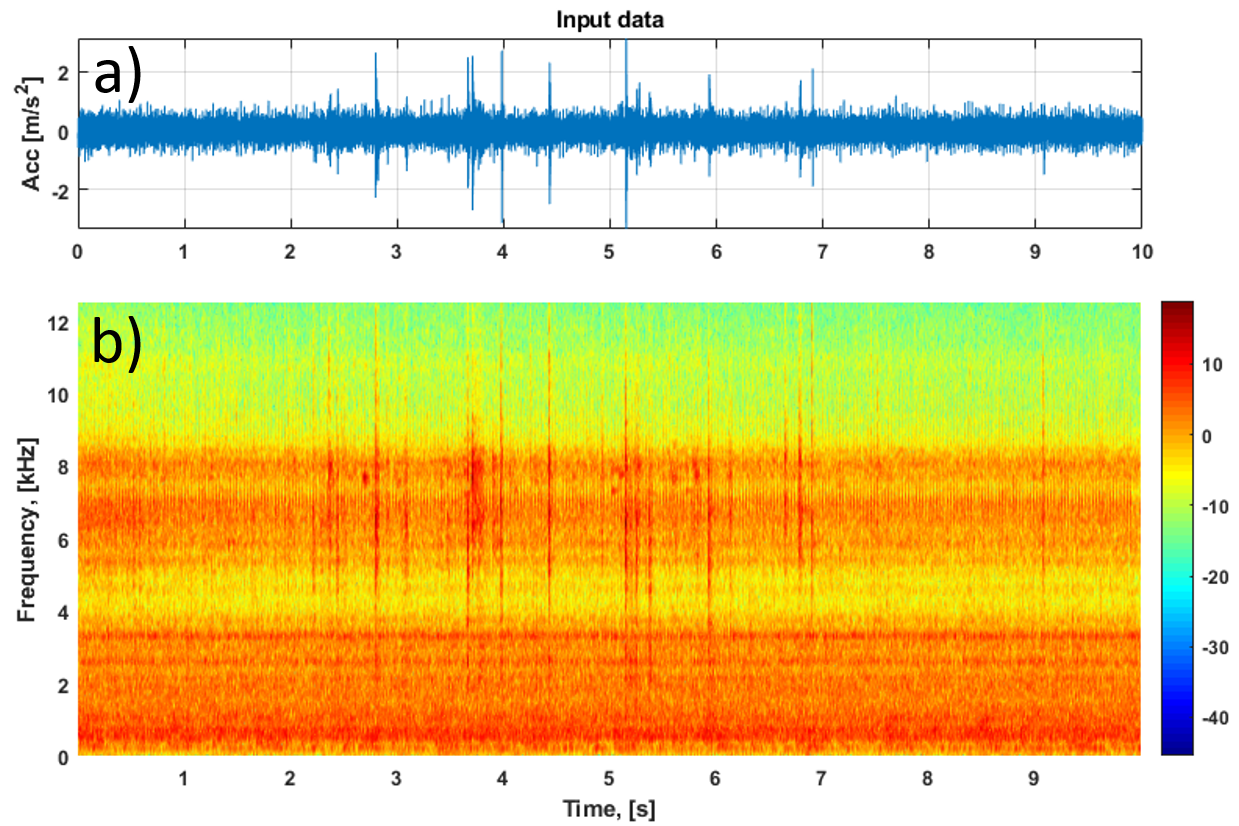
\includegraphics[width=.8\textwidth]{figs/raw.png}
\caption{Raw vibration data (a) and time-frequency representation (b).}
\label{fig:raw_signal_all}
\end{figure}

In the beginning the spectrogram is factorized using the $\beta$-HALS NMF algorithm. The obtained base and encoding matrices are presented in Fig. \ref{fig:NMF_matrix}. To demonstrate that second encoding feature describes properly recognized cyclic component the zoomed fragment is presented in Fig. \ref{fig:NMF_zoom}.

\begin{figure}[ht!]
\centering
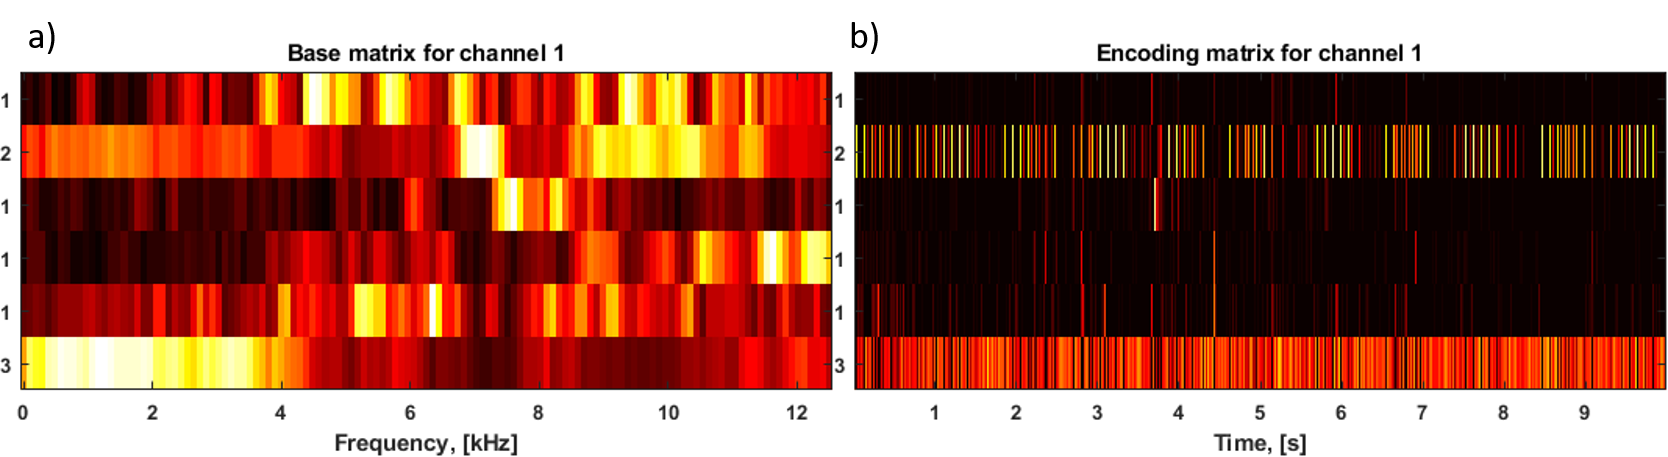
\includegraphics[width=.85\textwidth]{figs/mats.png}
\caption{Base (a) and encoding (b) matrices with individual features labeled with the cluster assignment.}
\label{fig:NMF_matrix}
\end{figure}

\begin{figure}[ht!]
\centering
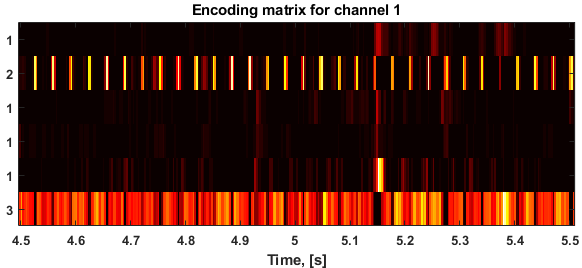
\includegraphics[width=0.65\textwidth]{figs/mats_zoom.png}
\caption{Zoom on short segment of encoding matrix.}
\label{fig:NMF_zoom}
\end{figure}

\begin{figure}[ht!]
\centering
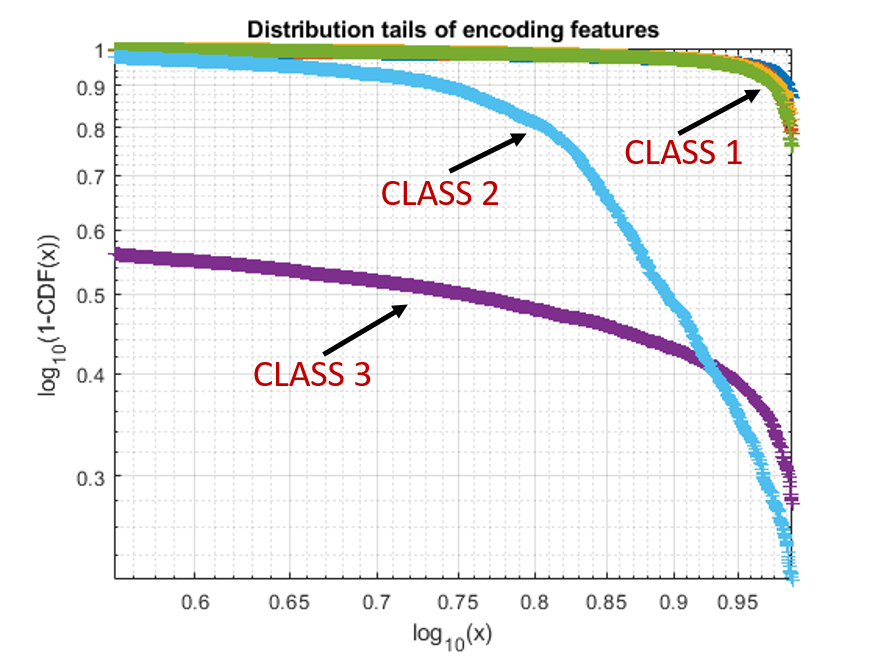
\includegraphics[width=0.65\textwidth]{figs/tails.png}
\caption{Distribution tails of the encoding features of NMF factorization. Tails are calculated in the normalized range of $(0.5,1)$. The value of clustering threshold calculated with the knee criterion of k-NN search $\varepsilon=2.25$. Based on that DBSCAN algorithm detected 3 clusters.}
\label{fig:NMF_tails}
\end{figure}

Then vectors from the encoding matrix are grouped based on clustering of their distribution tails with DBSCAN algorithm (see Fig. \ref{fig:NMF_tails}). It allows to establish differences between signal components and identify which features take part in describing every individual component. After that, features from the base and encoding matrix are selected and allow to form the new output base and encoding matrices for separate components of the signal. 

In the next step, waiting time analysis based on the encoding matrices allows to assign labels to the extracted components allowing to automatically classify them for the user as noise, non-cyclic impulsive component (denoted here as artifacts) and, what is the most important, the component describing the fault (see Fig. \ref{fig:NMF_hist}).


\begin{figure}[ht!]
\centering
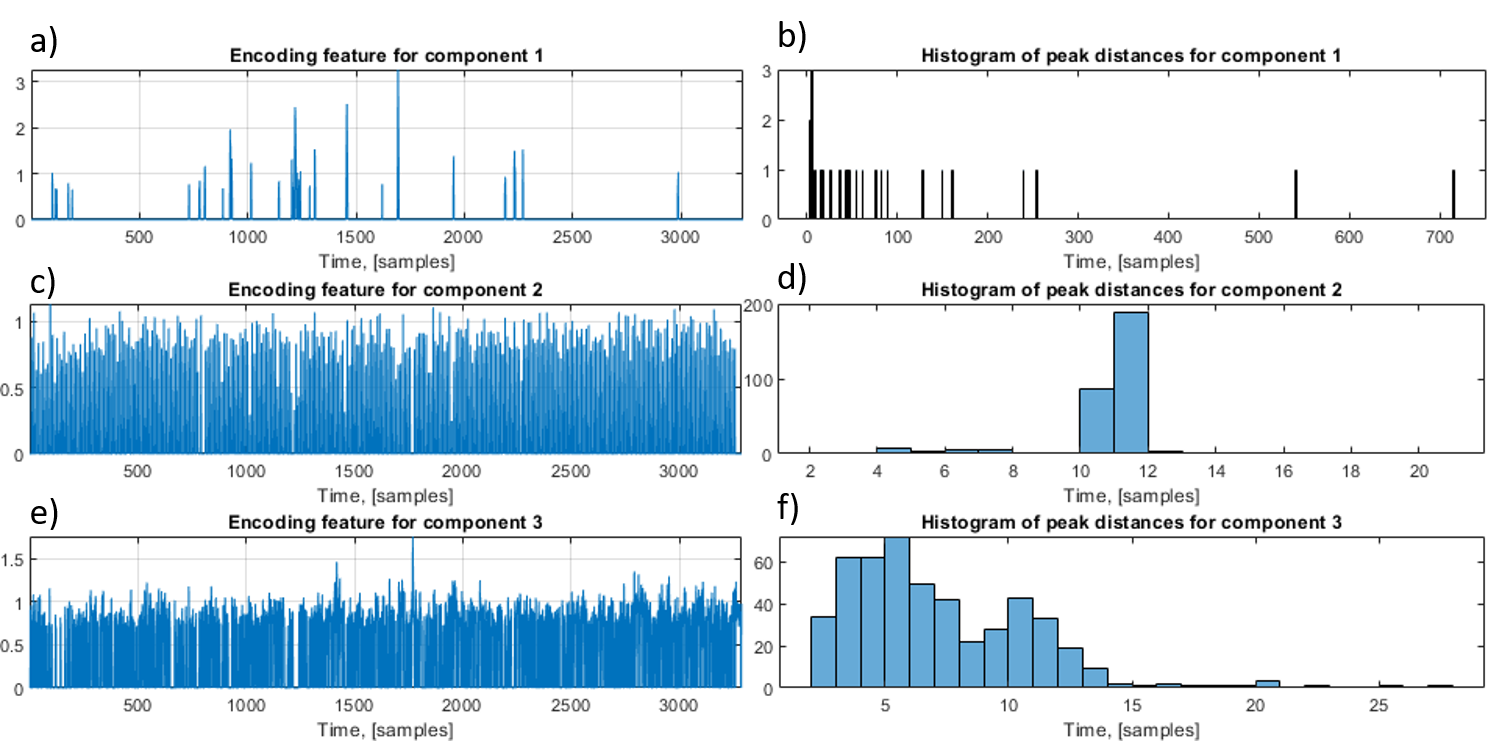
\includegraphics[width=\textwidth]{figs/hist.png}
\caption{Encoding features of discovered components (a,c,e) and peak distance distributions in those (b,d,f). Distances are calculated for peaks higher than 20\% of the maximum value. Analysis of those histograms allowed to determine that top panels describe the artifact component, middle ones -- damage component, and bottom ones -- noise component.}
\label{fig:NMF_hist}
\end{figure}



\begin{figure}[ht!]
\centering
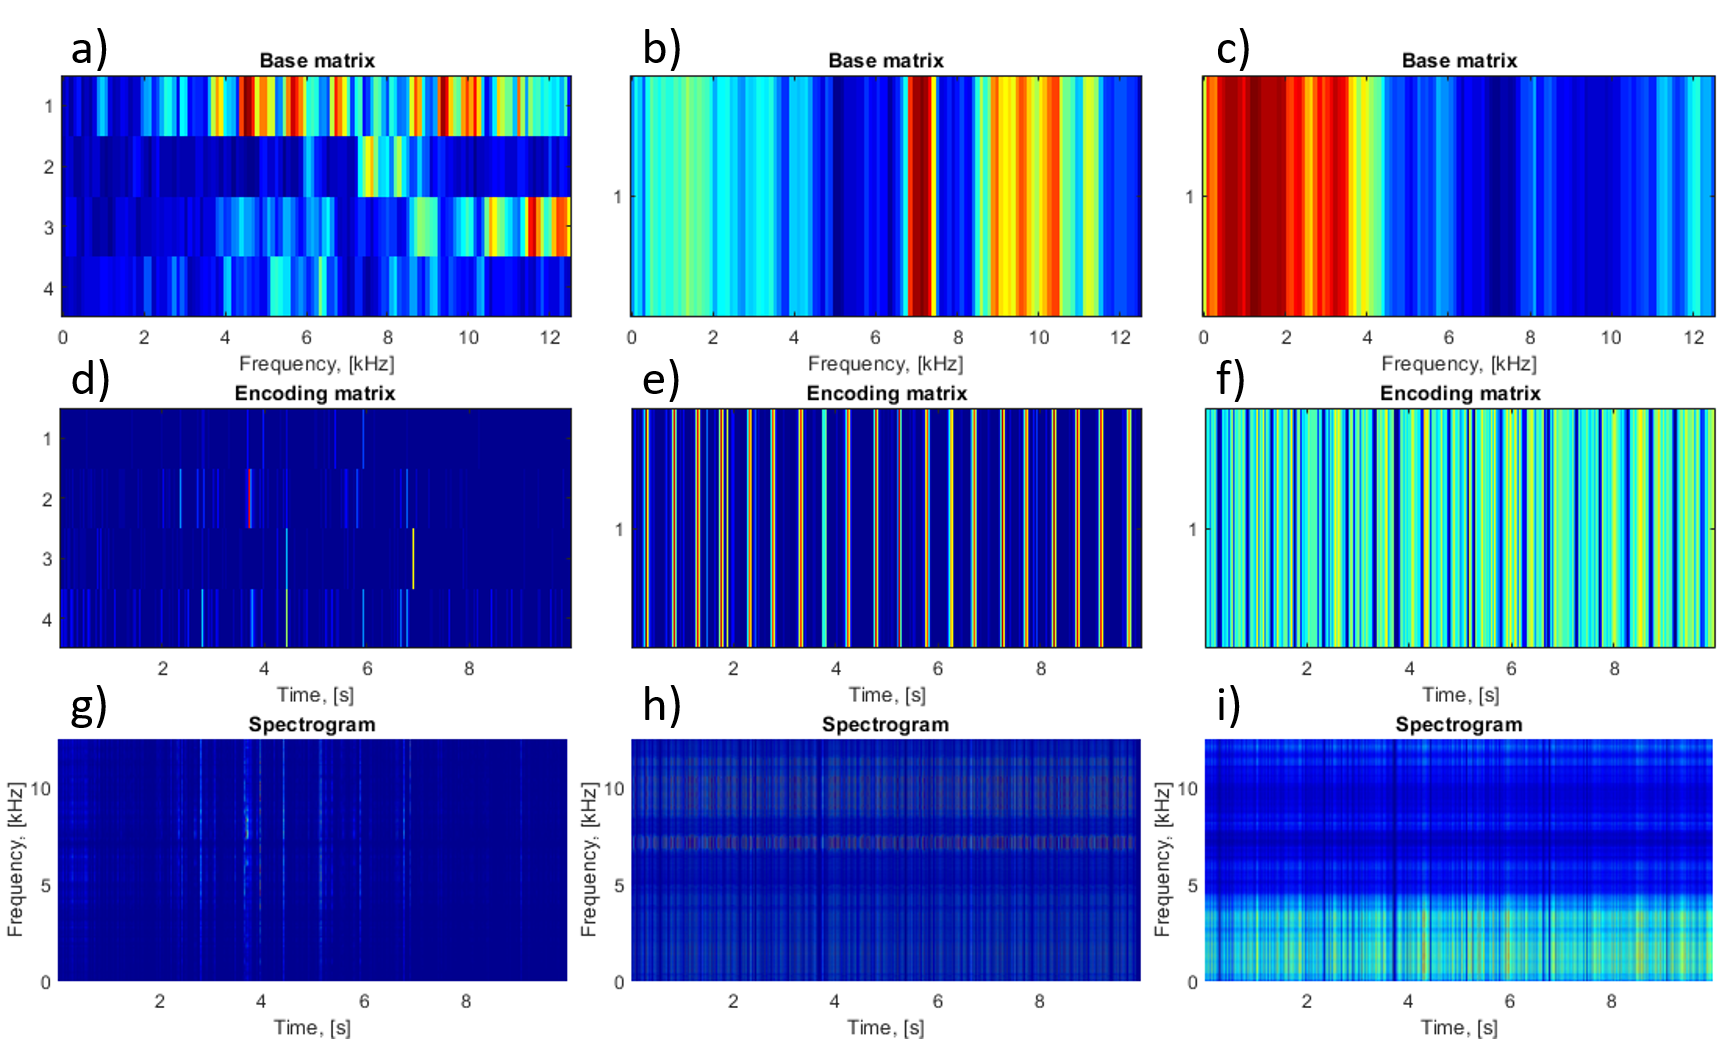
\includegraphics[width=.9\textwidth]{figs/res.png}
\caption{Feature matrices reconstructed for all components (a-f) with corresponding recovered magnitude spectrograms (g-i). Panels a,d,g describe structures for artifact component, panels b,e,h for damage component, and panels c,f,i for noise component.}
\label{fig:NMF_result}
\end{figure}

\begin{figure}[ht!]
\centering
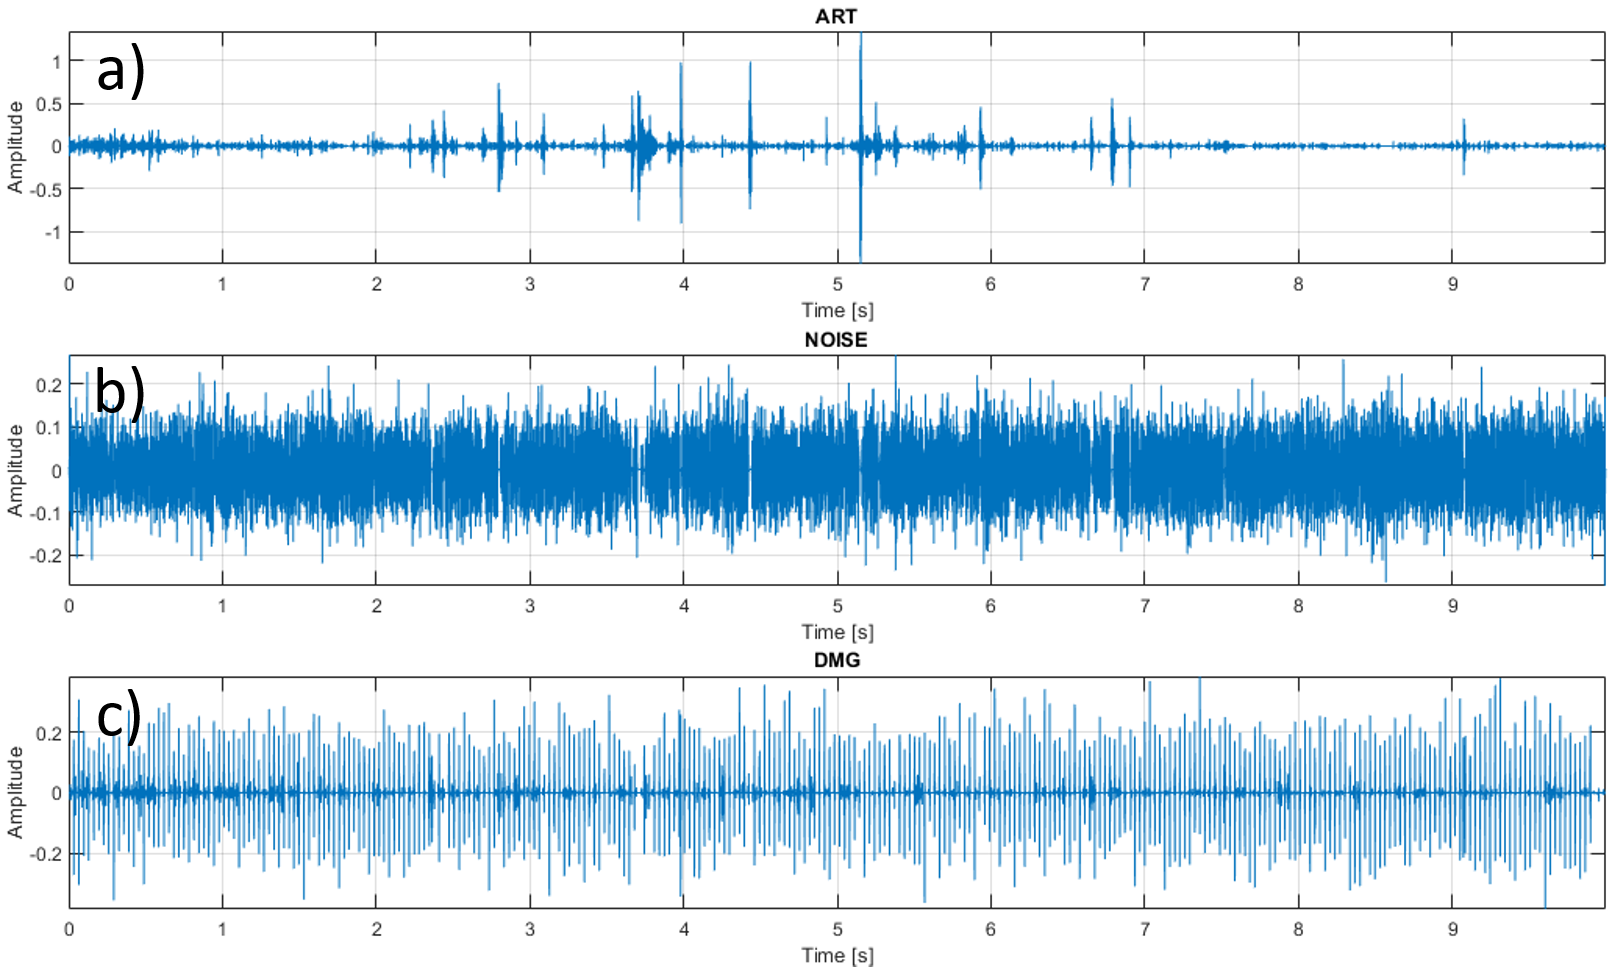
\includegraphics[width=.95\textwidth]{figs/out.png}
\caption{Separate components extracted from the signals.} 
\label{fig:NMF_out}
\end{figure}

\begin{figure}[ht!]
\centering
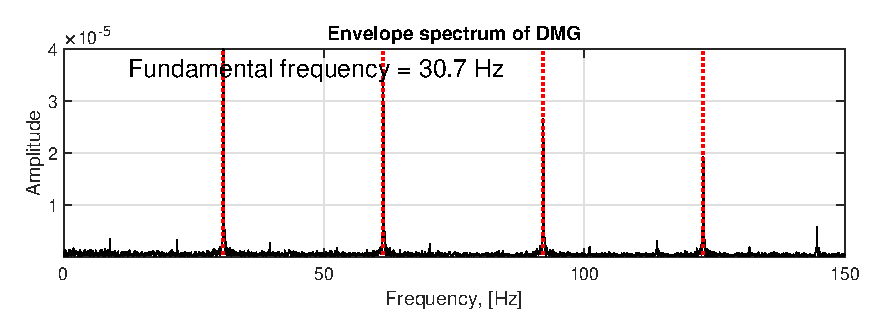
\includegraphics[width=.8\textwidth]{figs/spec.eps}
\caption{Envelope spectrum of fault-related component.}
\label{fig:NMF_outspec}
\end{figure}

When labels are assigned, base and encoding matrices are multiplied, and the magnitude spectrograms are obtained for each component (see Fig. \ref{fig:NMF_result}). Finally, Griffin-Lim algorithm is used to estimate the corresponding imaginary layer for the obtained component-specific spectrograms. It enables the reconstruction of time series for each component, which is only possible based on the full complex form of the STFT containing the imaginary layer describing the phase (see Fig. \ref{fig:NMF_out}). Then, envelope spectra of recovered components are evaluated to confirm their correct recovery (see Fig. \ref{fig:NMF_outspec}). As a result, both impulsive components have been properly recovered.

\subsection{Case 2: Data with no faults and impulsive noise}

The same methodology has been applied to the same signal without the added fault component. Such case is analyzed in order to verify if the presented method will properly separate and identify noise and random impulsive component when no fault component is present. It would be an additional value that the algorithm can not only find the damage when it is present, but also indicate that the machine is healthy when there are no fault-related components in the signal.

\begin{figure}[ht!]
\centering
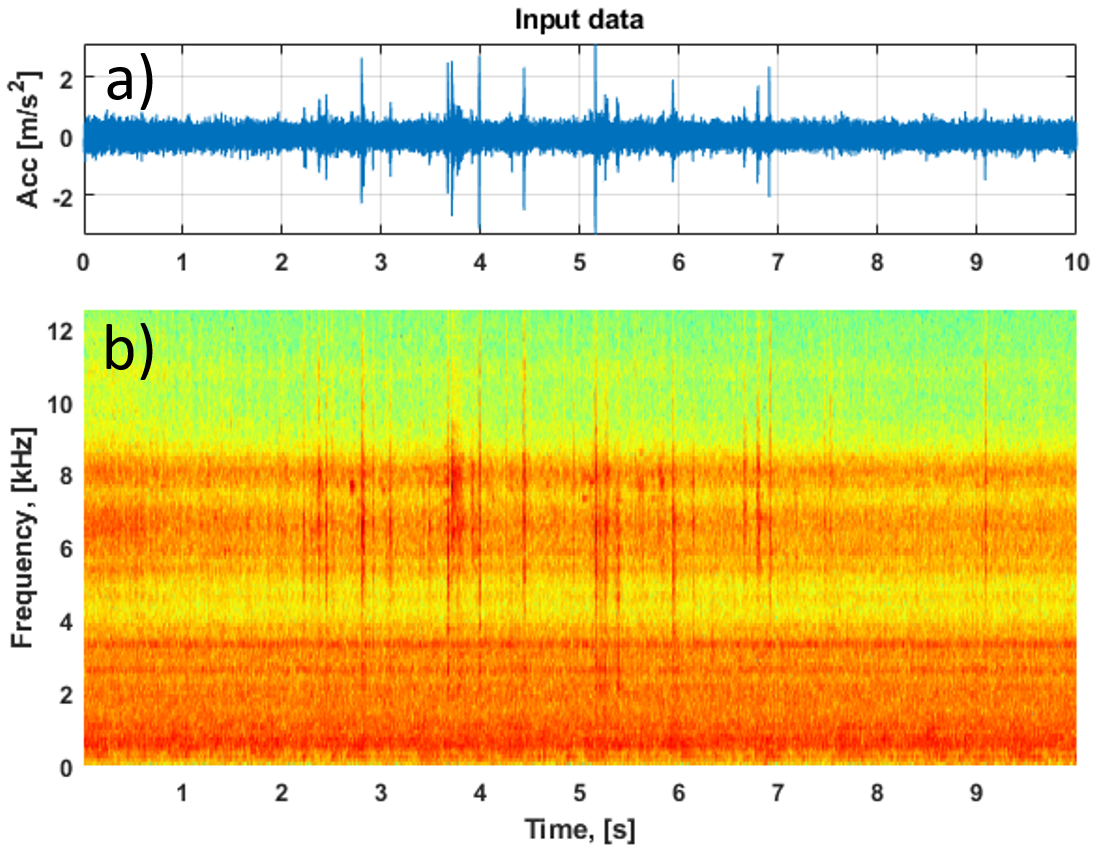
\includegraphics[width=0.8\textwidth]{figs/rawk.png}
\caption{Raw vibration data (a) and time-frequency representation (b).}
\label{fig:raw_signal_k}
\end{figure}

Consequently to the previous case, in the first step spectrogram is calculated with the same parameters as for signal containing damage signature (see Fig. \ref{fig:raw_signal_k}). Authors want to emphasize that those and all other parameters of the algorithm remain the same for both cases to ensure fair comparison.

\begin{figure}[ht!]
\centering
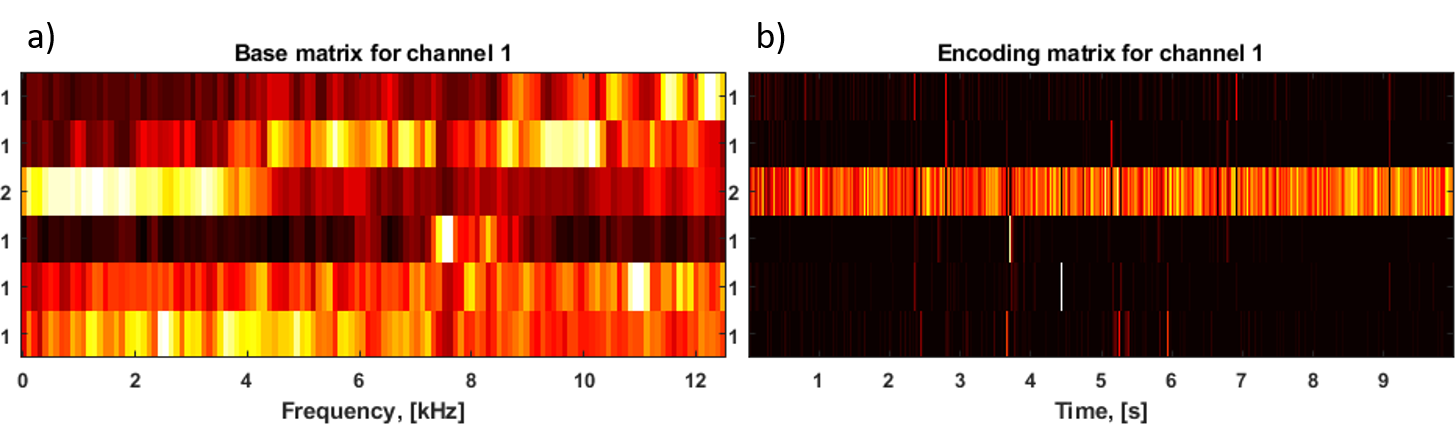
\includegraphics[width=0.85\textwidth]{figs/matsk.png}
\caption{Base (a) and encoding (b) matrices with individual features labeled with the cluster assignment.}
\label{fig:NMF_matrixk}
\end{figure}

Fig. \ref{fig:NMF_matrixk} presents the results of spectrogram factorization. Features are then classified, and as one can see in the labels of the vectors of base and encoding matrix, DBSCAN discovered two separate classes among the features. Tails of encoding features calculated for the grouping process are presented in Fig. \ref{fig:NMF_tailsk}.

\begin{figure}[ht!]
\centering
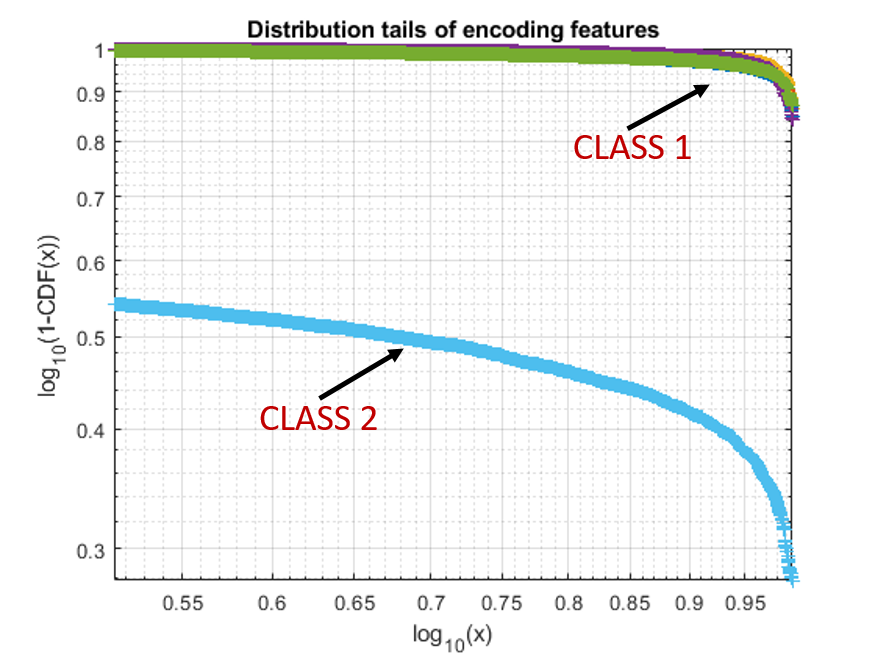
\includegraphics[width=0.7\textwidth]{figs/tailsk.png}
\caption{Distribution tails of the encoding features of NMF factorization. Tails are calculated in the normalized range of $(0.5,1)$. The value of clustering threshold calculated with the knee criterion of k-NN search $\varepsilon=0.94$. Based on that DBSCAN algorithm detected 2 clusters.}
\label{fig:NMF_tailsk}
\end{figure}

\begin{figure}[ht!]
\centering
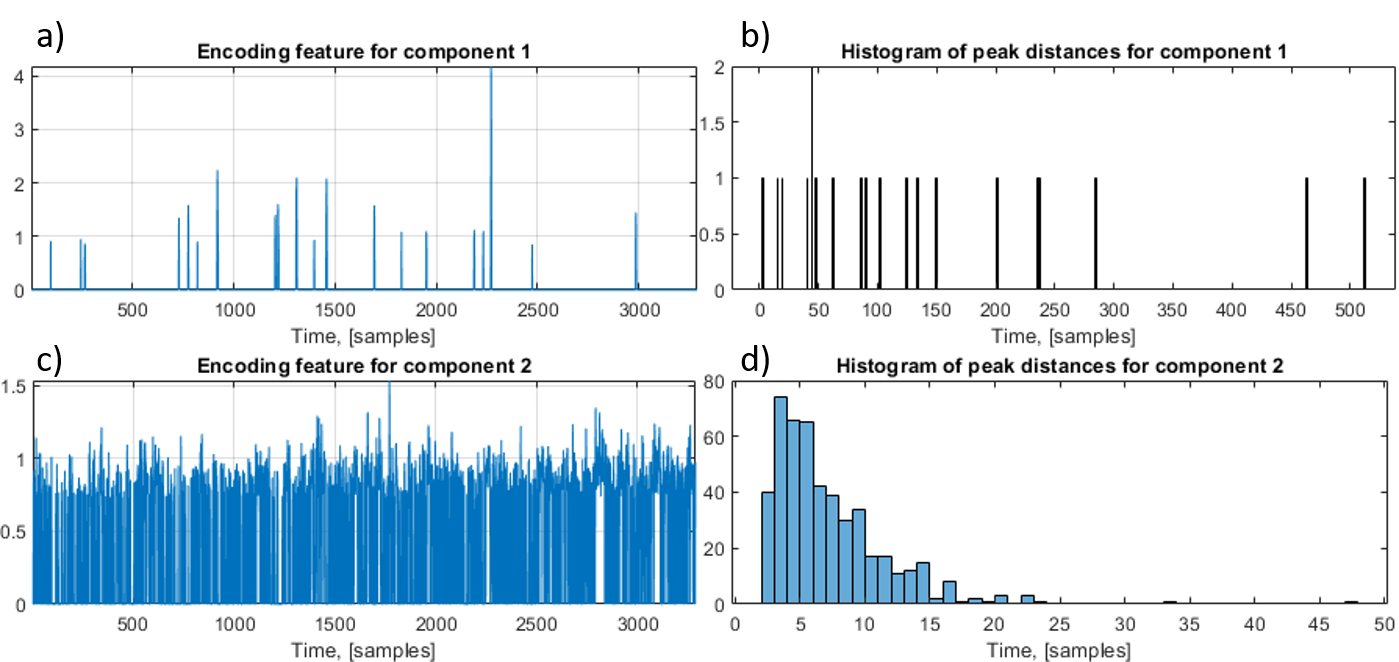
\includegraphics[width=\textwidth]{figs/histk.png}
\caption{Encoding features of discovered components (a,c) and peak distance distributions in those (b,d). Distances are calculated for peaks higher than 20\% of the maximum value. Analysis of those histograms allowed to determine that panels a,b describe the artifact component, and panels c,d -- noise component.}
\label{fig:NMF_histk}
\end{figure}


\begin{figure}[ht!]
\centering
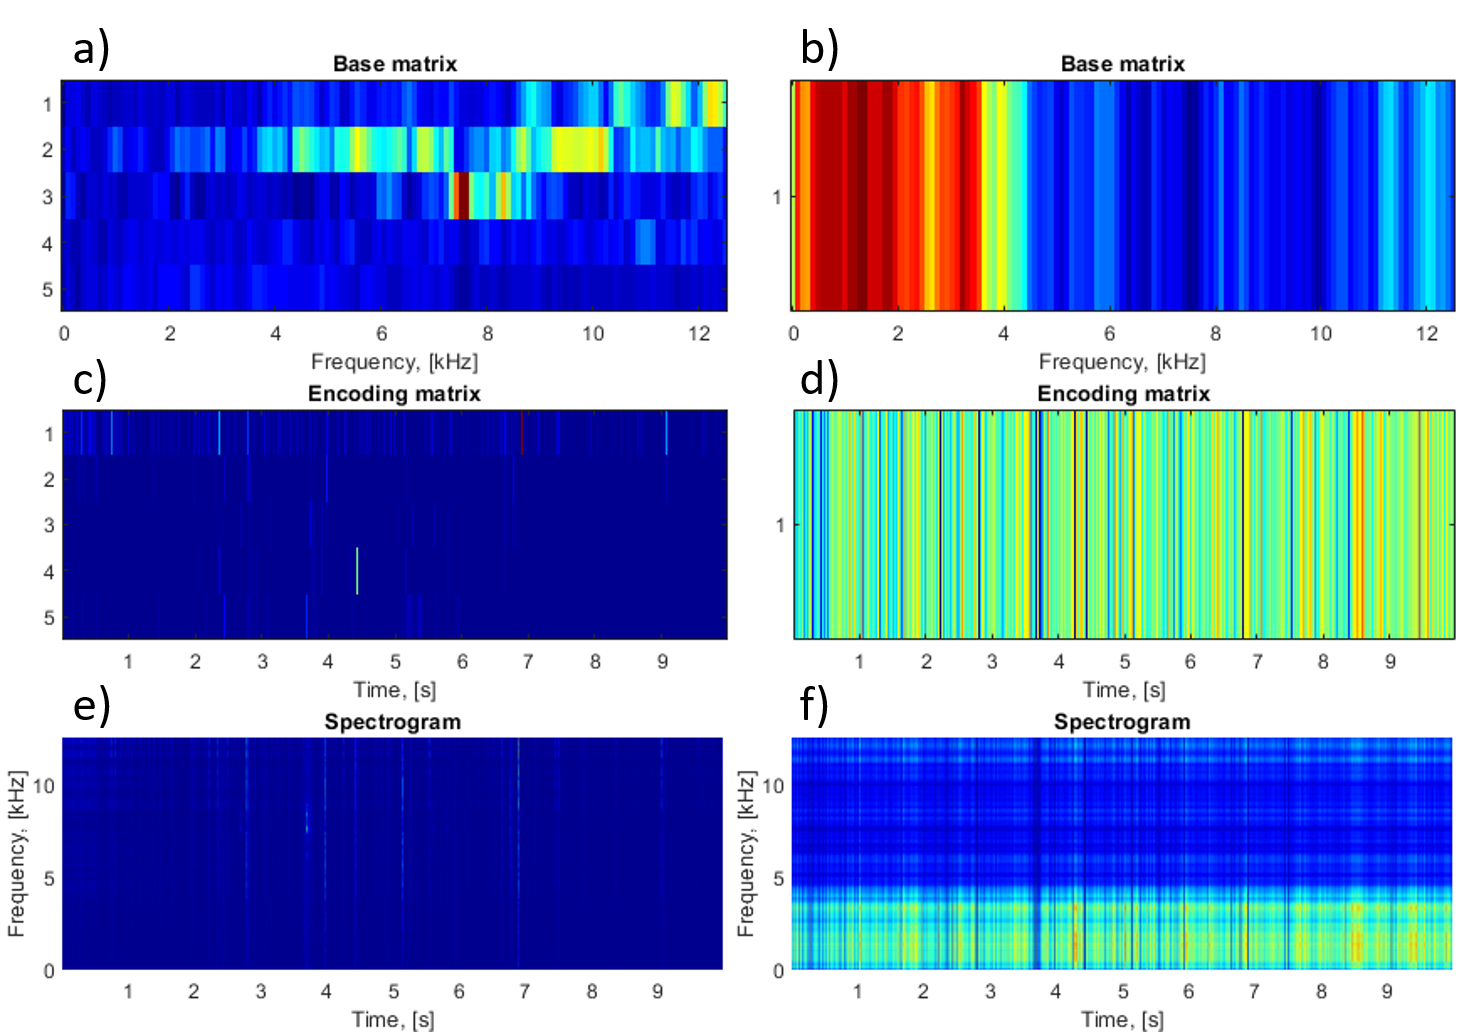
\includegraphics[width=\textwidth]{figs/resk.png}
\caption{Feature matrices reconstructed for all components (a-d) with corresponding recovered magnitude spectrograms (e,f). Panels a,c,e describe structures for artifact component, and b,d,f for noise component.}
\label{fig:NMF_resultk}
\end{figure}

Based on the result of feature grouping, the elementary base and encoding matrices are constructed, each component is labeled based on waiting time analysis (see Fig. \ref{fig:NMF_histk}) and the  multiplication of feature matrices allows to reconstruct the magnitude spectrograms (see Fig. \ref{fig:NMF_resultk}). Then their phase layers are estimated with Griffin-Lim algorithm and individual time series for each component can be reconstructed (see Fig. \ref{fig:NMF_outk}). In the end waiting times analysis allows to label the components as noise and random impulses denoted as artifacts.



\begin{figure}[ht!]
\centering
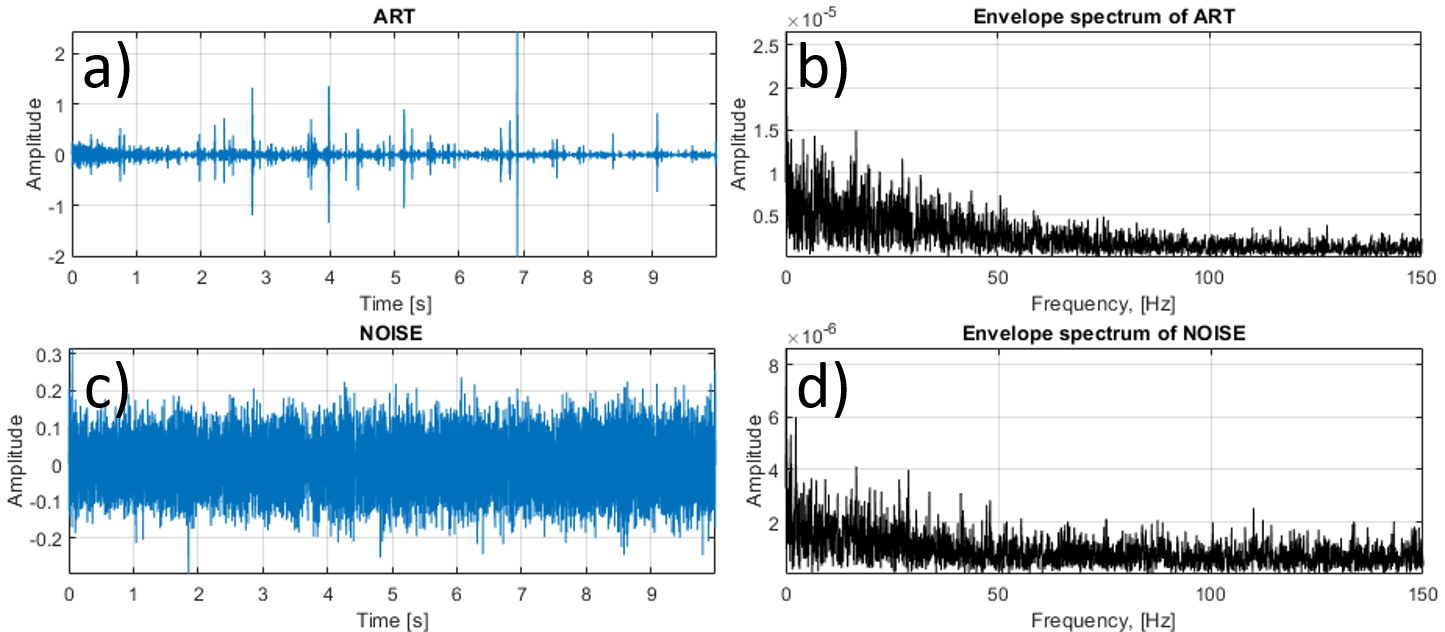
\includegraphics[width=0.8\textwidth]{figs/outk.png}
\caption{Separate components extracted from the signals along with their envelope spectra.}
\label{fig:NMF_outk}
\end{figure}

\section{Discussion}\label{disc}




Most of local damage detection procedures are focused on detection of impulses in time domain, time-frequency domain or finding hidden periodicity of the informative signals. Results of those procedures are just information that there is a fault present in the signal, with possible identification of faulty elements or a knowledge how to design a filter to extract the signal of interest, such as for Kurtogram, Spectral Kurtosis etc. In case of searching for an impulsive signal hidden in Gaussian noise, most of the methods work very well.

Unfortunately, when non-Gaussian noise appears in the acquired signal, which sometimes can be highly energetic and impulsive, signal processing becomes much more complicated. It can happen both from theoretical point of view (usage of many techniques is not allowed) as well as practically - because a given method is not able to detect a damage, or properly isolate it. The concept of infogram developed by Antoni seems to be an optimal way of signal processing in such context \cite{antoni2016info}. The infogram is looking on both impulsiveness of squared envelope and its periodicity via envelope spectrum. Hence, it should recognise non-cyclic impulses as impulsive but not periodic component, interpreting such component as not related to the fault.


Authors tried to compare the results with other known techniques, however none of them returned acceptable results for different reasons.

\begin{itemize}
    \item Before deciding to use $\beta$-HALS NMF authors investigated the possibility of using one of several different NMF algorithms that are computationally simpler, such as Classic NMF, Convex NMF, Semi-Binary NMF and HALS NMF \cite{cichocki2009nonnegative}. Unfortunately, none of them was able to produce feature matrices that presented the acceptable level of separability between the vectors, which was manifested either by missing impulses or by leaked noise information in the encoding vectors describing cyclic impulsive component related to the fault. Hence, if NMF could not produce correct features, all of the subsequent steps of the algorithm are irrelevant. Additionally, $\beta$-HALS NMF has been used because of its reliability. It originates from the fact that $\beta$-divergence used as a cost function has different properties than mean square error used in classic implementations. In this form the performance as well as convergence is significantly better than for the classic NMF. Besides, $\beta$-HALS NMF model is less susceptible to noise and produces closer fit than classic NMF \cite{cichocki2008flexible}. 
    \item Frequency-domain analysis such as usage of selectors, exhibits different problem. It is focused on selecting some part of frequency spectrum, so if two impulsive components occupy the same frequency band, they are not separable by those methods. However, if the goal is not to separate the components but to be able to see the fault at all, even as multiple components mixed within one signal, frequency-domain analysis can still be helpful.
    \item Cyclostationary analysis is another approach to discovering cyclic component in the signal. Authors made an attempt to use bi-frequency map called Cyclic Spectral Coherence as a base representation for the analysis. Sadly, high-energy non-cyclic impulsive component influenced the calculations significantly enough to corrupt the entire map, and information about the cyclic content was not visible at all.
    \item Authors also considered machine learning or deep learning techniques for component separation. Regrettably, this type of signal is very rare and there is no dataset that could serve for any form of learning. Hence, this approach has been disregarded.
\end{itemize}




The developed method also utilizes two perspectives: first of the NMF feature matrices is indicating the location of information in frequency domain, and the second one clusters the frequency content related to this information from time perspective. Processing of resulting classes allows to reconstruct the individual components as a final result. The great benefit of spectrogram factorization that using the combined perspective, one may extract SOI even if cyclic and non-cyclic impulses exist in the same frequency range.

From signal processing perspective proposed procedure can be described as source separation. It is possible to extract signal of interest but also source related to non-cyclic disturbances that describe other process. In practice, the second impulsive component does not have to be non-cyclic, i.e. it can also describe another fault. In fact, not many other techniques developed in last decade operate in that way. The advantages of NMF-based signal processing has been recently presented in \cite{wodecki2019impulsive}. In this paper authors focused on automation of the procedure and new interesting use case (with the same frequency band for cyclic and non-cyclic impulses) that is very hard to deal with using classical techniques.

However, there is one aspect of the method that functions as an input parameter and in the ideal case could be automated. It is the NMF rank, which is still provided by the user. In this application authors used the value of 6 for a specific reason. In general one can expect that such vibration signal can contain a noise component that is, generally speaking, time-invariant in the short term and will form one of the classes. Next one or two classes are assumed for fault components (occurrence of more than 2 different faults in the same time in one machine is extremely unlikely). This makes three classes. However, in case of machines experiencing random impacts, such as the ore crusher, the non-cyclic impulsive component emerges, that is random in time and energy. The random aspect of the energy of those impacts makes the impulses more or less wide in the frequency spectrum. Because of that, NMF algorithm is not able to recognize those individual impulses to belong to the same class. This is why for those types of behaviors one has to provide more than one NMF class, and authors decided to provide at least three. Hence, assuming one noise class, two (at most) faults and three classes provided for random impulsive behavior such as described before, authors ended up with the amount of six total classes for NMF factorization, which is a general recommendation for using this algorithm. 

As one can see in the provided experimental analysis, in the case containing one fault there were four classes remaining for the random impacts and in the case without the fault there were five. In both cases the factorization process took advantage of the amount of classes and populated them all with parts of random impulsive process. The analysis of base matrices for the artifact class for each case (see Fig. \ref{fig:NMF_result} and Fig. \ref{fig:NMF_resultk}) shows that some of those parts (practically speaking: vectors of those base matrices) are very different from each other, which suggests that dividing this component into subclasses really allowed to provide more in-depth separation regarding the entire NMF process efficiency. 

Nevertheless, on top of all of this consideration, there is a need to automatically determine the amount of classes (the rank) for the spectrogram factorization. However, beside this aspect the proposed method is fully automatic in its operation, and presents
significant advantages, such as the possibility of separating multiple different impulsive components occupying the same frequency band.

\section{Conclusions}

A novel procedure for local damage detection in rolling element bearings in presence of impulsive noise is presented in the paper. The problem has been noticed recently and some interesting techniques have been proposed by several authors, however, novelty of this approach is related to specific situation. Namely, fault-related cyclic impulses and non-cyclic impulses describing impulsive noise occupy the same frequency band. In such a case all selector-based approaches applied in frequency domain are not efficient. They can at most improve signal to noise ratio but they are not able to extract signal of interest. Presented approach is based on time-frequency representation of the signal and takes advantage of both domains -- frequency and time. Using factorization of spectrogram matrix we are able to spatially classify and differentiate sources with different frequency and time properties in time-frequency domain.

In previous work we have already proposed NMF-based technique for local damage detection in bearings/gears for several contexts (two cyclic impulsive signals but with different frequency bands for both components, or multiple channels used for SOI extraction). The method presented here is based on application of NMF to spectrogram, density-based clustering of received features, automatic selection of number of classes, time-frequency domain reconstruction and phase estimation that allows to obtain time series of recovered components. Original contribution of this paper could be considered from two perspective. Firstly, frequency band occupied by non-cyclic impulsive source covers frequency band occupied by cyclic impulsive source. Secondly, using NMF for source clustering required some manual actions, and we proposed a way to automate it.

Presented technique has serious practical meaning. It has been developed for the heavy-duty ore crusher operating in mining industry, an example of critical infrastructure in the company. Using this approach we have detected local damage in rolling element bearing (fault frequency 30.7Hz). It should be highlighted, that for healthy case (no damage in the bearing) this method is able to properly classify sources and indicate that there is no fault-related component, even in the presence of impulsive noise.


\section*{Acknowledgments}
This activity has received funding from European Institute of Innovation and Technology (EIT), a body of the European Union, under the Horizon 2020, the EU Framework Programme for Research and Innovation. This work is supported by EIT RawMaterials GmbH under Framework Partnership Agreement No. 18253 (OPMO - Operational Monitoring of Mineral Crushing Machinery).
% \section*{References}

\bibliography{mybibfile}

\end{document}